\documentclass{article}
\usepackage{graphicx,fullpage}
\author{Pieter Vermeesch}
\title{{\tt Radial\-Plotter}: a Java application for fission track,
luminescence and other radial plots}
\begin{document}

\maketitle

Radial plots are bivariate (x$_j$,y$_j$) scatterplots where:

\begin{eqnarray}
x_j = 1/\sigma(z_j), & y_j = (z_j-z_0)/\sigma(z_j), & 
\mbox{~~~~ for 1  $\leq$ j  $\leq$ n}
\label{eq:xjyj}
\end{eqnarray}

with z$_j$ a transformation of some data and $\sigma(z_j)$ the
corresponding measurement uncertainty.  For example, if z$_j$ =
log(t$_j$) then $\sigma(z_j)$ = $\sigma(t_j)/t_j$.  z$_0$ is a
convenient central value such as the weighted mean.  The slope of a
line connecting the origin (x=0,y=0) of a radial plot with a data
point (x$_j$,y$_j$) equals $z_j$, and the horizontal distance along
x-axis is a measure if its precision.  Thus, the radial plot
simultaneously visualises a measurement's value and precision.  No
other graphical method achieves this goal with the same elegance
(Galbraith, 1988).  This makes the radial plot the method of choice
for visualising heteroscedastic data, i.e.  data with (large and)
variable measurement uncertainties.  Traditional applications in the
Earth Sciences are fission track and luminescence dating, which are
governed by Poisson processes (e.g., Galbraith, 1990; Galbraith et
al., 1999).  In principle, however, radial plots can be used for any
kind of data.\\

{\tt RadialPlotter} is a user-friendly application for generating
radial plots.  It has the following advantages over existing programs
such as {\tt Track\-key} or {\tt Mac\-Track}.  (1) The program was
developed solely for radial plots and does not perform other functions
for data reduction or interpretation. Therefore, radial plot functions
are not buried deep inside the menu structure and the interface is
very straightforward.  (2) {\tt RadialPlotter} was written in Java
(version 5) and is, therefore, perfectly platform independent. (3) In
addition to fission track radial plots, {\tt RadialPlotter} also
offers the possibility to generate radial plots for luminescence
dating, or any other kind of data such as (U-Th)/He or
$^{40}$Ar/$^{39}$Ar ages.\\

{\tt RadialPlotter} can be downloaded free of charge from {\tt
http://pver\-mees.andro\-pov.org/radial\-plotter}.  The program
consists of a single executable jar file ({\tt Radial\-Plotter.jar}).
This makes installation straightforward: it suffices to download and
open this file to run {\tt RadialPlotter}.  For testing purposes,
three example input files are provided on the website, one for each of
the three possible input formats (`Fission Tracks', `Luminescence' and
`Other').  The graphical output can be saved as either bitmap or
vector images, in a {\tt .png} or {\tt .pdf} format,
respectively. {\tt RadialPlotter} automatically performs a
$\chi^2$-test for statistical homogeneity of fission track data.  For
populations that have failed this test, the program implements the
mixture modeling algorithm of Galbraith and Green (1990)(Figure
\ref{fig:input-output}).  Data points can be colour-coded to show an
additional variable such as chemical composition or a kinetic
parameter. Colour-coding can also be a useful tool for double-dating,
which is rapidly gaining popularity in detrital studies (e.g.,
Campbell et al., 2005).  For example, the U-Pb ages of double-dated
zircons could be shown as colours on a (U-Th)/He radial plot.
Hopefully, this kind of flexibility will give the radial plot the
wider user base which it deserves. \\

\begin{figure}
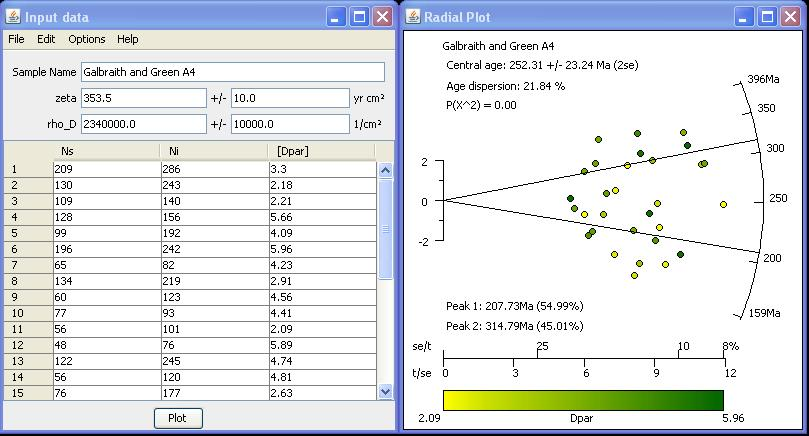
\includegraphics[width = \textwidth]{fig1.jpg}
\caption{Input (left) and output (right)  in the case of fission track
  dating.}
\label{fig:input-output}
\end{figure}

\section*{References}

\begin{description}

\item Campbell, I. H., Reiners, P. W., Allen, C. M.,
Nicolescu, S., Upadhyay, R., 2005:
He-Pb double dating of detrital zircons from the Ganges and Indus
Rivers: Implication for quantifying sediment recycling and
provenance studies, Earth and Planetary Science Letters 237, 402-432.

\item Galbraith,  R. F., 1988:  Graphical display of  estimates having
  differing standard errors, Technometrics, 30, 271-281.

\item Galbraith, R. F., 1990: The radial plot: graphical assessment of
  spread  in  ages, Nuclear  Tracks  and  Radiation Measurements,  17,
  207-214.

\item Galbraith, R. F. and Green, P. F., 1990: Estimating the component 
ages in a finite mixture, Nuclear Tracks and Radiation Measurements, 17, 
197-206.

\item  Galbraith, R.  F., Roberts,  R.  G., Laslett,  G. M.,  Yoshida,
  H. and  Olley, J.  M., 1999: Optical  dating of single  and multiple
  grains of quartz from Jinmium rock shelter, northern Australia: Part
  I,  experimental design  and statistical  models,  Archaeometry, 41,
  339-364.

\end{description}

\end{document}
